\section{Exploring Covariance Functions}


\subsection{Characteristics of covariance functions \cite{gp-ml}}


\subsubsection{Symmetry and positive semidefiniteness}
The inner product representation that any valid covariance matrix can produce is the form of a Gram matrix. Given a vector of input points ${X_i | i = 1, ..., n}$ and a covariance function $k$, a Gram matrix $K$ is the $n \times n$ matrix whose $(i,j)$-th entry is $k(x_i, x_j)$. This requires any proposed covariance matrix to exhibit the properties of a Gram matrix, namely symmetry and positive semidefiniteness.

\begin{equation*}
    \begin{aligned}
        K_{ij} = K_{ji} \\
        X^T K X \geq 0
    \end{aligned}
\end{equation*}

Symmetry is inherent from the inner product property since inner products are symmetric, i.e. $X_i^T X_j = X_j^T X_i$, and imposes $cov(X_i, X_j) = cov(X_j, X_i)$. $K$ satisfies positive semidefiniteness if, for any vector $V$ of inputs, $V^T K V \geq 0$. 
\begin{equation*}
    V^T K V = (K V)^T (K V) = ||K V||^2 \geq 0
\end{equation*}
This means that the covariance matrix must not produce negative variances for any linear combination of inputs.

\subsubsection{Varying the length scale}
Our covariance functions has some hyperparameters, e.g. the full form of SE in one dimension contains some free parameters $\sigma^2_f$, $\sigma^2_n$, and $l$:
\begin{equation*}
    k_y(x,x') = \sigma^2_f \exp\left(-\frac{1}{2}\frac{|x - x'|^2}{l^2}\right) + \sigma^2_n\delta_{x,x'}
\end{equation*}
Note that our covariance function is for $k_y$ as it is for the noisy targets $y$, not the function $f$. $\sigma^2_f$ is the signal variance, which controls the overall scale of the function. $\sigma^2_n$ is the noise variance, which controls the amount of noise in the observations. $\delta_{X,X'}$ is the Kronecker delta which represents our independence of noise assumption.

$l$ is a "length scale" hyperparameter that controls how sensitive our functions are - if we specify a lower $l$, we can "artificially" get a high $k(X,X')$. One way to determine $l$ is by the expected number of "upcrossings" that our kernel is expected to make for a given level $u$. A function performs an upcrossing for $u$ when $u = f(x)$ and $dy/dx > 0$. For example, with $u = 2$ and $y = x^2$, there exists one upcrossing at $(2, \sqrt{2})$ where $dy/dx = 4$, and a downcrossing at $(2, -\sqrt{2})$ where $dy/dx = -4$. For our zero-mean Gaussian processes, the expected number of upcrossings of our (stationary) kernel for a level $ 0 < u < 1$ is:
\begin{equation*}
    \mathbb{E}[N_u] = \frac{1}{2\pi} \sqrt{\frac{-k''(0)}{k(0)}} \exp \left(-\frac{u^2}{2k(0)}\right)
\end{equation*}
We can empirically count the number of upcrossings between 0 and 1 and set this equal to the expected number of upcrossings to get a value for $l$:
\begin{equation} \label{eq:general_l}
    \frac{1}{2\pi} \sqrt{\frac{-k''(0)}{k(0)}} \exp \left(-\frac{u^2}{2k(0)}\right) = \hat{N}_u
\end{equation}

A large amount of upcrossings implies our data-generating function wiggles rapidly, so our $l$ becomes smaller to produce a covariance function that in turn produces more flexible functions.

\subsubsection{Mean square continuity and differentiability}
To understand how smooth the functions drawn from a Gaussian process are, we need to understand how differentiable and continuous they are. A more differentiable function implies that the function contains higher order polynomials which makes it smoother, and a continuous function avoids any reductions in smoothness produced by discontinuities.

Because the functions drawn from the Gaussian distribution are random functions between datapoints, there are infinitely many possible functions and determining if they are all continuous or differentiable is impossible. TODO 

% We are l Instead, we can examine if the covariance function responsible for producing these functions is differentiable and continuous.

% The quadratic term in our limit means our mean squared errors will also vary continuously, so we avoid wild "swings" in uncertainty when moving away from training data points in the input space. More importantly, it allows the error term to be expanded directly into kernel terms: 

\paragraph{Continuity}
Let $x$ be an infinite-length vector of inputs $x_1, x_2, ...$ whose values linearly approach some stable fixed point $x_*$ as the sequence progresses. Formally:
\begin{equation*}
    \lim_{k \to \infty} |x_k - x_*| = 0
\end{equation*}

A regular function $f$ is continuous at $x_*$ if three conditions are met. $x_*$ must exist in the domain of $f$, e.g. $f(X) = 1/x$ is not continuous at $f(0)$ because $0$ is not in the domain of $f$. There must be a single limit the function approaches.
\begin{equation*}
    f(X) = \begin{cases}
        0 & \text{if } X < 0 \\
        1 & \text{if } X > 0 \\
        2 & \text{if } X = 0
    \end{cases}
\end{equation*}
In this example, at $f(0)$ $x$ is not continuous at $x = 0$ since $f$ approaches both $0$ and $1$. This single limit needs to be the same as the function evaluation at the limit. If we removed the $0 \text{ if } X < 0$ case to produce a single limit, it would still not be continuous at $x = 0$ since the limit would be $1$ but $f(0) = 2$. Formally summarising these three ideas:
\begin{equation*}
    \lim_{x \to x_*} |f(x) - f(x_*)| = 0
\end{equation*}

A Gaussian process $f$ is MS continuous at $x_*$ if the expected function evaluations $E[f(x)]$ quadratically approach $f(x_*)$ as $x \to x_*$. Formally:
\begin{equation*}
    \lim_{x \to x_*} \mathbb{E}[(f(x) - f(x_*))^2] = 0
\end{equation*}

Thanks to the quadratic term, we can expand our error term directly into kernel terms. The covariance function $k$ is defined as the expected value of the product of two function evaluations:
\begin{equation*}
    \begin{aligned}
        \mathbb{E}[(f(x) - f(x_*))^2] = \mathbb{E}[f(x)^2] + \mathbb{E}[f(x_*)^2] - 2\mathbb{E}[f(x)f(x_*)] \\
        = k(x, x) + k(x_*, x_*) - 2k(x, x_*)
    \end{aligned}
\end{equation*}
Using this expansion in our definition of MS continuity: 
\begin{equation} \label{eq:ms_continuity}
    \lim_{x \to x_*} | k(x, x) - 2k(x, x_*) + k(x_*, x_*) | = 0
\end{equation}
Because $x_*$ is given, $k(x_*, x_*)$ is a constant. This limit requires that both $k(x, x)$ and $k(x, x_*) \to k(x_*, x_*)$ as $x \to x_*$, which is the very definition of continuity of $k$ at $x_*$ - they guarantee that $x_*$ is in the domain of $k$, that it has a single limit, and this limit of $k(x, x_*)$ is $k(x_*, x_*)$ as $x \to x_*$. Therefore, a Gaussian process is MS continuous at $x_*$ if and only if the covariance function $k$ is continuous at $x_*$.  

\paragraph{Differentiability}
$f$ is MS differentiable at $x_*$ in the $i$th direction of our input vector $X$ if:
\begin{equation*}
    \lim_{h \to 0} \mathbb{E} \left[| \frac{(f(x_* + h e_i) - f(x_*))}{h} - \frac{\partial f}{\partial x_{*i}}(x_*) |\right]^2 = 0
\end{equation*}
$e_i = (0_0, ..., 0_{i-1}, 1_i, 0_{i+1}, ..., 0_n)$ is a unit vector that constrains the change in $x$ to only the $i$th dimension. We assume $m(x_*) = 0$ for simplicity, but a non-zero mean does not change the structure of this proof and leads to the same result.

Expanding and creating simplifying $A$ and $B$ terms to represent the limit and the proposed derivative respectively:
\begin{equation*}
    \begin{aligned}
        \lim_{h \to 0} \mathbb{E} \left[(A_h - B)^2\right] = \mathbb{E}[A_h^2] + \mathbb{E}[B^2] - 2\mathbb{E}[A_h B] = 0 \\
        A_h = \frac{f(x_* + h e_i) - f(x_*)}{h} \\
        B = \frac{\partial f}{\partial x_{*i}}(x_*)
    \end{aligned}
\end{equation*}
Similar to MS continuity, we expand $A_h^2$ into kernel terms:
\begin{equation} \label{eq:msd_a}
    \mathbb{E}[A_h^2] = \frac{1}{h^2} \left( k(x_* + h e_i, x_* + h e_i) + k(x_*, x_*) - 2k(x_* + h e_i, x_*) \right)
\end{equation}
$k(x_*,x_*)$ is a constant, but the other terms vary with $h$. We can use a second-order Taylor series to approximate these terms if $k$ is twice continuously differentiable at $x_*$. Starting with the univariate $k(x_* + h e_i, x_*)$:
\begin{equation*}
    \begin{aligned}
        k(x_* + h e_i, x_*) = \\
        k(x_*, x_*) \\
        + h [\partial_{u_i}k](x_*, x_*) \\
        + \frac{h^2}{2} [\partial_{u_i u_i}^2k] (x_*, x_*) \\
        + O(h^3)
    \end{aligned}
\end{equation*}
$u_i$ and $v_i$ denote the first $x_* + h e_i$ and second $x_*$ arguments respectively in the $i$th direction. TODO explain $O$ and why it's in terms of $h^3$
Then, the multivariate $k(x_* + h e_i, x_* + h e_i)$:
\begin{equation*}
    \begin{aligned}
        k(x_* + h e_i, x_* + h e_i) = \\
        k(x_*, x_*) \\
        + h [\partial_{u_i}k + \partial_{v_i}k](x_*, x_*) \\
        + \frac{h^2}{2} [\partial_{u_i u_i}^2 k + \partial_{u_i v_i}^2 k + \partial_{v_i v_i}^2 k](x_*, x_*) \\
        + O(h^3) 
    \end{aligned}
\end{equation*}
Substituting these approximations into \ref{eq:msd_a}:
\begin{equation*}
    \begin{aligned}
        \mathbb{E}[A^2_h] = \frac{1}{h^2} \\
        k(x_*, x_*) + k(x_*, x_*) - 2k(x_*, x_*) \\
        + h [\partial_{u_i}k + \partial_{v_i}k](x_*, x_*) - 2h[\partial_{u_i}k](x_*, x_*) \\
        + \frac{h^2}{2} [\partial_{u_i u_i}^2 k + \partial_{u_i v_i}^2 k + \partial_{v_i v_i}^2 k](x_*, x_*) - 2\frac{h^2}{2} [\partial_{u_i u_i}^2k](x_*, x_*) \\
        + O(h^3)
    \end{aligned}
\end{equation*}
The constant $k(x_*, x_*)$ terms cancel and the $O(h^3)$ remainders combine but remain the same order. 

We can combine the linear partial derivatives to form a single function $[\partial_{u_i}k + \partial_{v_i}k - 2\partial_{v_i}k]$. Thanks to the symmetry of the covariance matrix inherited from the Gram matrix, $k(u,v) = k(v,u)$ and $\partial_{u_i}k = \partial_{v_i}k$ and substituting in either into our linear term cancels it completely. 

Similarly, we can combine the quadratic derivatives:
\begin{equation*}
    E[A^2] = \frac{1}{h^2} \frac{h^2}{2}[\partial_{u_i u_i}^2 k + \partial_{u_i u_i}^2 k + \partial_{v_i v_i}^2k](x_*,x_*) - h^2[\partial_{u_i v_i}^2 k](x_*, x_*)
\end{equation*}
Cancelling $\frac{1}{h^2}$ and $\frac{h^2}{2}$ and simplifying:
\begin{equation*}
    \begin{aligned}
    = [\partial_{u_i v_i}^2 k + \partial_{u_i u_i}^2 k + \partial_{v_i v_i}^2k - \partial_{u_i v_i}^2 k](x_*, x_*) \\
    = [\partial_{u_i u_i}^2 k + \partial_{u_i v_i}k - \partial_{v_i v_i}^2 k](x_*, x_*)
    \end{aligned}
\end{equation*}
Similarly to the linear terms, using the symmetry of $k$ to cancel $\partial_{u_i u_i}^2$ and $\partial_{v_i v_i}^2$ yields the final expression for $\mathbb{E}[A_h^2$:
\begin{equation} \label{eq:msd_a_final}
    \mathbb{E}[A_h^2] = \partial_{u_i v_i}^2 k(x_*,x_*) + O(h^3) 
\end{equation}

Because $B$ is Gaussian, its square is simply its variance:
\begin{equation*}
    \begin{aligned}
        \mathbb{E}[B^2] = \text{Var}\left(\frac{\partial f}{\partial x_{*i}}(x_*)\right) \\
        = \text{Cov} \left(\frac{\partial f}{\partial x_{*i}}(x_*), \frac{\partial f}{\partial x_{*i}}(x_*) \right) \\
    \end{aligned}
\end{equation*}
We can substitute our regular limit definition of differentiability outside of MS space, with different small increments $h$ and $h'$:
\begin{equation*}
    = \text{Cov} \left(\frac{f(x_* + h e_i) - f(x_*)}{h}, \frac{f(x_* + h' e_i) - f(x_*)}{h'} \right)
\end{equation*}
The $h$ and $h'$ denominators merely scale the covariance, so we can take them out of the covariance expression:
\begin{equation*}
    = \frac{1}{hh'} \text{Cov} \left(f(x_* + h e_i) - f(x_*), f(x_* + h' e_i) - f(x_*) \right)
\end{equation*}
Using additivity TODO explain:
\begin{equation*}
    \mathbb{E}[B^2] = \frac{1}{hh'} \left( k(x_* + h e_i, x_* + h' e_i) - k(x_*, x_* + h' e_i) - k(x_* + h e_i, x_*) + k(x_*, x_*) \right)
\end{equation*}
We already have $k(x_* + h e_i, x_*)$ from \ref{eq:uni_taylor_a} directly, and $k(x_*, x_* + h e_i)$ by symmetry and substituting $h'$ for $h$. Our multivariate Taylor series $k(x_* + h e_i, x_* + h' e_i)$ looks similar to \ref{eq:multi_taylor_a}:
\begin{equation*}
    \begin{aligned}
        k(x_* + h e_i, x_* + h' e_i) = \\
        k(x_*, x_*) \\
        + h [\delta_{u_i}k](x_*, x_*) 
        + h' [\delta_{v_i}k](x_*, x_*) \\
        + \frac{h^2}{2} [partial_{u_i u_i}^2k](x_*, x_*) \\
        + hh' [\partial_{u_i v_i}^2k](x_*, x_*) \\
        + \frac{h'^2}{2} [\partial_{v_i v_i}^2k](x_*, x_*) \\
        + O(||(h,h')||^3)
    \end{aligned}
\end{equation*}

Substituting these results into $\mathbb{E}[B^2]$:
\begin{equation*}
    \begin{aligned}
        \mathbb{E}[B^2] = \frac{1}{hh'} \\
        k(x_*,x_*) \\
        + k(x_*,x_*) + k(x_*,x_*) - k(x_*,x_*) \\
        + h [\delta_{u_i}k](x_*, x_*) - h [\delta_{u_i}k](x_*, x_*) \\
        + h' [\delta_{v_i}k](x_*, x_*) - h' [\delta_{v_i}k](x_*, x_*) \\
        + \frac{h^2}{2} [\partial_{u_i u_i}^2k](x_*, x_*) -  \frac{h^2}{2} [\partial_{u_i u_i}^2k](x_*, x_*) \\
        + hh' [\partial_{u_i v_i}^2k](x_*, x_*) \\
        + \frac{h'^2}{2} [\partial_{v_i v_i}^2k](x_*, x_*) - \frac{h'^2}{2} [\partial_{v_i v_i}^2k](x_*, x_*) \\
        + O(h^3) + O(h'^3) + O(||(h,h')||^3) \\
    \end{aligned}
\end{equation*}
All constant, linear $h$ and $h'$, and $h^2$ and $h'^2$ terms cancel, leaving the mixed term and the remainders. $\frac{1}{hh'}$ cancel and the remainders can be combined since TODO:
\begin{equation} \label{eq:msd_b_final}
    \mathbb{E}[B^2] = \partial_{u_i v_i}^2 k(x_*, x_*) + O(h^2)
\end{equation}

For $\mathbb{E}[A_h B]$, assuming zero-mean:
\begin{equation*}
    \mathbb{E}[A_h B] = \text{Cov} \left( \frac{f(x_* + h e_i) - f(x_*)}{h}, \frac{\partial f}{\partial x_{*i}}(x_*) \right)
\end{equation*}
Similarly to $B$, we can remove the scaling factor $\frac{1}{h}$:
\begin{equation*}
    = \frac{1}{h} \text{Cov} \left( f(x_* + h e_i) - f(x_*), \frac{\partial f}{\partial x_{*i}}(x_*) \right)
\end{equation*}
By linearity of covariance TODO elabourate:
\begin{equation*}
    = \frac{1}{h} \left[ \text{Cov} (f(x_* + h e_i), \frac{\partial f}{\partial x_{*i}}(x_*) ) - \text{Cov} (f(x_*), \frac{\partial f}{\partial x_{*i}}(x_*)) \right]
\end{equation*}

A fundamental identities for Gaussian fields TODO elabourate is:
\begin{equation*}
    \begin{aligned}
        \text{Cov}(f(u), \delta_{u_i} f(v)) = \delta_{u_i} k(u, v) \\
    \end{aligned}
\end{equation*}
Applying it to both terms:
\begin{equation*}
    \begin{aligned}
        \text{Cov}(f(x_* + h e_i), \frac{\partial f}{\partial x_{*i}}(x_*)) = \delta_{u_i} k(x_* + h e_i, x_*) \\
        \text{Cov}(f(x_*), \frac{\partial f}{\partial x_{*i}}(x_*)) = \delta_{v_i} k(x_*, x_*) \\
    \end{aligned}
\end{equation*}

Taylor expanding our first term:
\begin{equation*}
    \begin{aligned}
        \delta_{u_i} k(x_* + h e_i, x_*) = \\
        \delta_{u_i} k(x_*, x_*) \\
        + h \delta_{u_i v_i}^2 k(x_*, x_*) \\
        + \frac{h^2}{2} \delta_{u_i u_i u_i}^3 k(x_*, x_*) \\
        + O(h^3) \\
    \end{aligned}
\end{equation*}
We can take advantage of symmetry of $k$ to cancel out the constant term using the second term in $\mathbb{E}[A_hB]$ - when $u = v$, $\delta_{v_i} k(x_*, x_*) = \delta_{u_i} k(x_*, x_*)$. Substituting this into $\mathbb{E}[A_h B]$:
\begin{equation*}
    \begin{aligned}
        \mathbb{E}[A_h B] = \frac{1}{h} \\
        h \delta_{u_i v_i}^2 k(x_*, x_*)
        + \frac{h^2}{2} \delta_{u_i u_i v_i}^3 k(x_*, x_*) \\
        + O(h^3) \\
    \end{aligned}
\end{equation*}

Dividing by $h$ reduces the order of the remainder. Simplifying for a final expression:
\begin{equation} \label{eq:msd_ab_final}
    \mathbb{E}[A_h B] = \delta_{u_i v_i}^2 k(x_*, x_*) + \frac{h}{2} \delta_{u_i u_i u_i}^3 k(x_*, x_*) + O(h^2)
\end{equation}

Substituting \ref{eq:msd_a_final}, \ref{eq:msd_b_final}, and \ref{eq:msd_ab_final} into our original limit definition of MS differentiability:
\begin{equation*}
    \lim_{h \to 0} \delta_{u_i v_i}^2 k(x_*, x_*) + O(h^3) + \delta_{u_i v_i}^2 k(x_*, x_*) + O(h^2) - 2 \left( \delta_{u_i v_i}^2 k(x_*, x_*) + \frac{h}{2} \delta_{u_i u_i u_i}^3 k(x_*, x_*) + O(h^2) \right) = 0 
\end{equation*}
Redefining $A = \delta_{u_i v_i}^2 k(x_*, x_*)$ and $B = \frac{h}{2} \delta_{u_i u_i v_i}^3 k(x_*, x_*)$ for brevity:
\begin{equation*}
    \lim_{h \to 0} A + O(h^3) + A + O(h^2) - 2(A + \frac{h}{2}B + O(h^2)) = 0
\end{equation*}
Expanding the last term:
\begin{equation*}
    \lim_{h \to 0} A + O(h^3) + A + O(h^2) - 2A - hB - 2O(h^2) = 0
\end{equation*}
All $A$ terms cancel. Combining and reducing the remainders to the lowest order:
\begin{equation*}
    \lim_{h \to 0} hB + O(h) = 0
\end{equation*}
We can aborsb $hB$ into $O(h)$ since it is a linear term in $h$:
\begin{equation} \label{eq:ms_differentiability}
    \begin{aligned}
        \lim_{h \to 0} O(h) = 0 \\
    \end{aligned}
\end{equation}
$O(h)$ approaches $0$ as $h \to 0$, so our limit definition of MS differentiability is met using a second-order Taylor expansion. We can extend this to any $k$-th derivative in MS space by using a $2k$-th order Taylor expansion of the covariance functions, which requires the covariance function to be $2k$-times continuously differentiable at $x_*$.

\subsection{Stationary GPs \cite{gp-ml}}

\subsubsection{Stationarity and isotropicism}
A stationary covariance function $k(X - X')$ is some function of $X - X'$ , and is invariant to the exact locations of $X$ and $X'$. An isotropic covariance function $k(|X - X'|)$ is a function of $|X - X'|$, and is is invariant to the direction of $X - X'$. For example, SE \cite{eq:se} is both stationary and isotropic because it is a function of $|X - X'|$.


% \subsubsection{Eigenfunction analysis of covariance functions}

\subsubsection{Stationary GPs in MS space}
Putting the stationary kernel $k(x,x') = k(x - x')$ into \ref{eq:ms_continuity}:
\begin{equation*}
    \lim_{x \to x_*} | k(x - x) - 2k(x - x_*) + k(x_* - x_*) | = 0
\end{equation*}
Simplifying the terms inside the kernels and combining like terms:
\begin{equation*}
    \lim_{x \to x_*} 2 | k(0) - k(x - x_*) | = 0
\end{equation*}
$2$ is a constant factor and can be ignored. Because $ | k(0) - k(x - x_*) |$ is invariant to direction, we can swap them to align with the definition of continuity at 0:
\begin{equation*}
    \lim_{x \to x_*} | k(x_* - x) - k(0) | = 0
\end{equation*}
Thus, a stationary covariance function is MS continuous at $x_*$ if and only if it is continuous at $x_* = 0$. Similarly, it can be shown that stationary covariance functions are MS differentiable at $x_*$ if and only if they are MS differentiable at $x_* = 0$.

\subsubsection{TODO Spectral density}
Bochner's theorem states that a complex-valued function is the covariance function of a 

It can be shown \cite{Gikhman2004-wc} that the covariance function of a stationary process can be represented as the Fourier transform of a positive finite measure.

\subsection{Stationary covariance functions \cite{gp-ml}}

\subsubsection{Squared exponential (SE)}
Here is the already introduced SE:
\begin{equation*}
    k(X,X*) = \exp \left(- \frac{|X - X'|^2}{2l^2} \right)
\end{equation*}

This covariance function is infinitely differentiable at $x - x' = 0$ thanks to the squared difference between $X$ and $X'$ in the exponent, so a GP using SE is infinitely mean-squared differentiable which produces extremely smooth functions.  

\paragraph{From feature space to SE}
We can derive this form by expanding $X$ into our feature space $\phi$ defined by Gaussian-shaped basis functions centred densely in $X$. Defining this basis function:
\begin{equation*}
    \phi_c(x) = \exp \left(- \frac{|x - c|^2}{2l^2} \right)
\end{equation*}
$c$ the centre of our basis functions. With our familiar isotropic Gaussian prior on the weights $W \sim \mathcal{N}(0, \sigma^2_pI)$, we get our familiar covariance function in weight-space:
\begin{equation*}
    k(x, x') = \sigma_p^2 \sum_{c=1}^N \phi_c(x) \phi_c(x') 
\end{equation*}
$N$ represents the number of these basis functions. If $N = \infty$ with centres everywhere between some interval $c_{min}$ and $c_{max}$, we can simply integrate over the interval:
\begin{equation*}
    \lim_{N \to \infty} \sigma_p^2 \sum_{c=1}^N \phi_c(x) \phi_c(x') = \sigma_p^2 \int_{c_{min}}^{c_{max}} \phi_c(x) \phi_c(x') dc
\end{equation*}
Plugging in our basis function:
\begin{equation*}
    k(x, x') = \sigma_p^2 \int_{c_{min}}^{c_{max}} \exp \left(- \frac{|x - c|^2}{2l^2} \right) \exp \left(- \frac{|x' - c|^2}{2l^2} \right) dc
\end{equation*}
Combining the exponentials:
\begin{equation*}
    = \sigma_p^2 \int_{c_{min}}^{c_{max}} \exp \left(- \frac{|x - c|^2 - |x' - c|^2}{2l^2} \right) dc
\end{equation*}
Expanding the squared terms, rearranging the fraction and simplifying:
\begin{equation*}
    = \sigma_p^2 \int_{c_{min}}^{c_{max}} \exp \left( -\frac{1}{l^2} \left[ c^2 - c(x + x') + \frac{x^2 + x'^2}{2} \right] \right) dc
\end{equation*}
We can complete the square on the $c$ terms to get a product of two exponentials:
\begin{equation*}
    = \sigma_p^2 \int_{c_{min}}^{c_{max}} \exp \left( -\frac{1}{l^2} \left[ (c - \frac{x + x'}{2})^2 - \frac{(x + x')^2}{4} \right] \right) dc
\end{equation*}
Our second term in the exponential does not vary with $c$ and can be safely factored out of the integral:
\begin{equation*}
    = \sigma_p^2 \exp \left( \frac{(x + x')^2}{4l^2} \right) \int_{c_{min}}^{c_{max}} \exp \left( -\frac{1}{l^2} (c - \frac{x + x'}{2})^2 \right) dc
\end{equation*}
If we let our $c_{min}$ and $c_{max}$ approach infinity, we can use the standard Gaussian integral:
\begin{equation*}
    \int_{-\infty}^{\infty} \exp \left( -\frac{1}{l^2} (c - \frac{x + x'}{2})^2 \right) dc = l\sqrt{\pi}
\end{equation*}
Substituting this in:
\begin{equation*}
    k(x, x') = \sigma_p^2 l\sqrt{\pi} \exp \left( -\frac{(x - x')^2}{4l^2} \right)
\end{equation*}
We can absorb the $l\sqrt{\pi}$ into the $\sigma_p^2$ term to produce our familiar SE with a $\sqrt{2}$ longer length scale:
\begin{equation*}
    k(x, x') = \sigma^2_p \exp \left( -\frac{(x - x')^2}{2(\sqrt{2}l)^2} \right)
\end{equation*}

\paragraph{Length scale in SE}
We can observe the role $l$ plays in SE by finding the value for $l$ analytically and rearranging it for $\hat{N}_u$ to see its effect on smoothness.

Using \ref{eq:general_l}:
\begin{equation*}
    l = \frac{1}{2\pi\hat{N}_u} \exp\left(-\frac{u^2}{2\sigma^2}\right)
\end{equation*}
Setting $u = 0$ makes our term inside the exponential equal to zero:
\begin{equation*}
    l = \frac{1}{2\pi\hat{N}_u}
\end{equation*}
Rearranging for $\hat{N}_u$:
\begin{equation*}
    \hat{N}_u = \frac{1}{2\pi l}
\end{equation*}
Here, $l$ behaves as a length scale - a larger $l$ reduces the number of upcrossings, stretching out the features over longer distances and producing smoother sample paths.


\begin{figure}[H]
    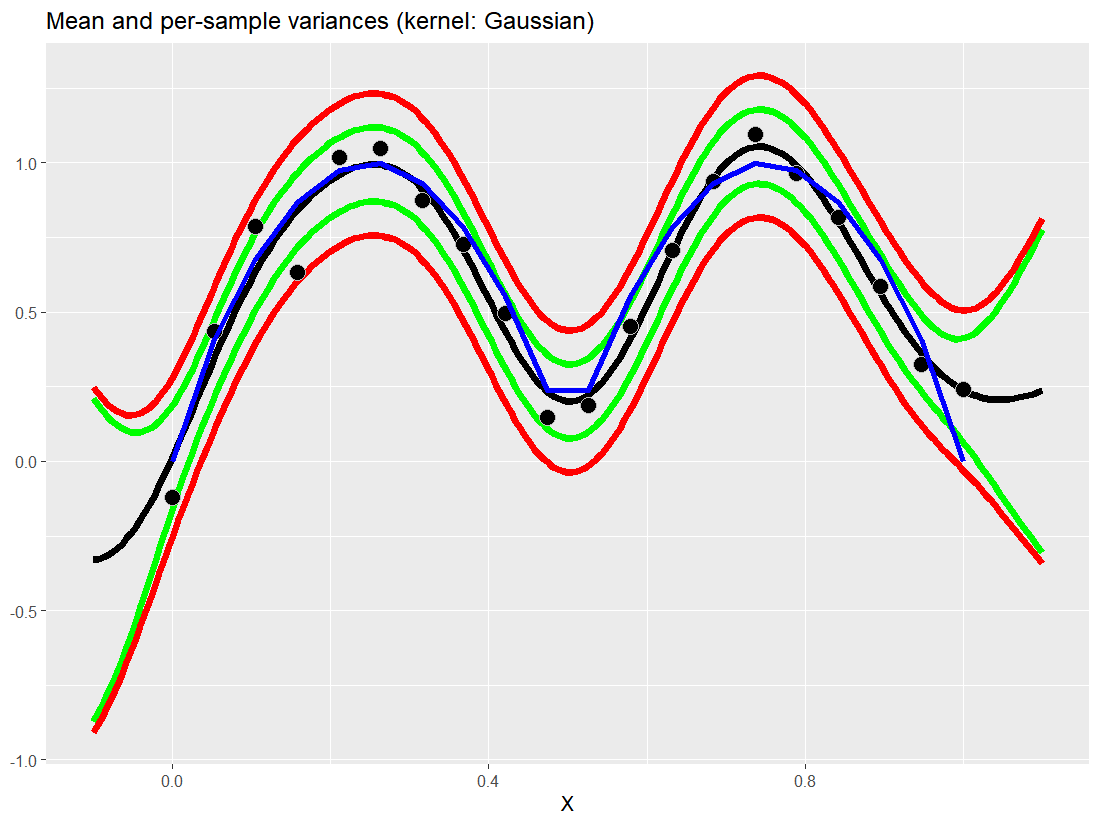
\includegraphics[height=0.5\textwidth]{gaussian_variances.png}
    \caption{
        Plot of a Gaussian process using SE applied to a toy dataset. The toy dataset ($n = 15$) is a data-generating function in blue with some Gaussian noise applied to produce the datapoints in black. The black line represents the expected function from the Gaussian process. The green line represents the 90\% confidence interval around the predictive distribution without the $\sigma^2_n$ term, representing the uncertainty surrounding predictions of the noise-free mean function $f(X)$. The red line represents the 90\% confidence interval with $\sigma^2_n$, representing the uncertainty surrounding predictions of the noisy observations $y$. \\
        TODO explain
    }
\end{figure}

\begin{figure}[H]
    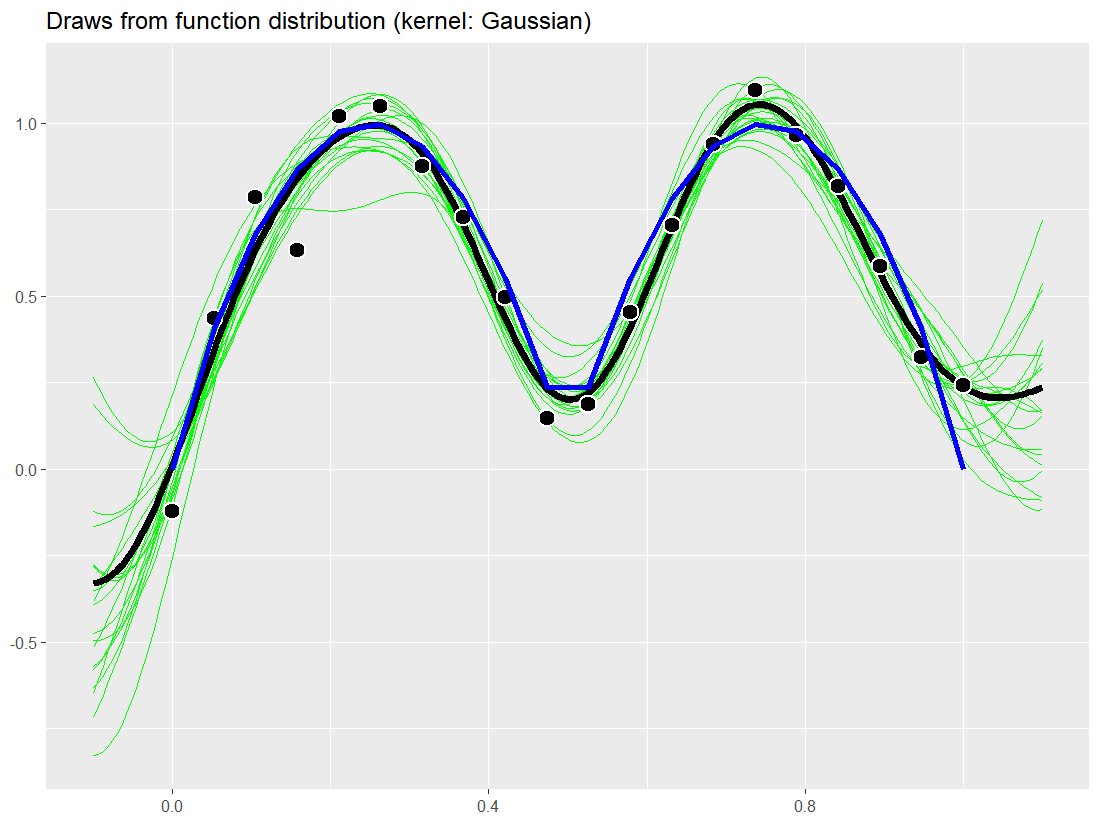
\includegraphics[height=0.5\textwidth]{gaussian_draws.png}
    \caption{
        Plots of functions from a Gaussian process using SE applied to the same toy dataset. The blue line and black datapoints and lines are as before, but the green lines here are a sample of functions drawn from the Gaussian process. \\
        TODO explain
    }
\end{figure}

\subsubsection{TODO Rational quadratic}
The rational quadratic can be seen as an infinite sum of SE with different length-scales.

TODO formulas

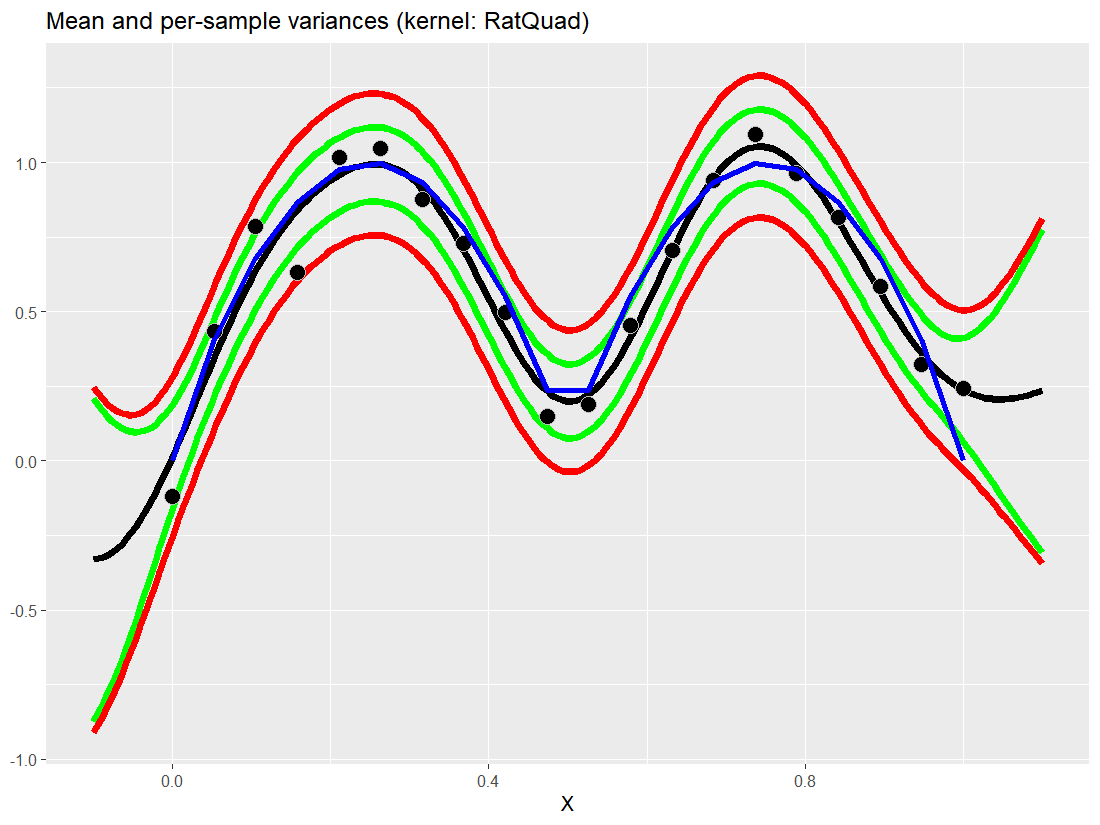
\includegraphics[height=0.5\textwidth]{ratquad_variances.png} \\
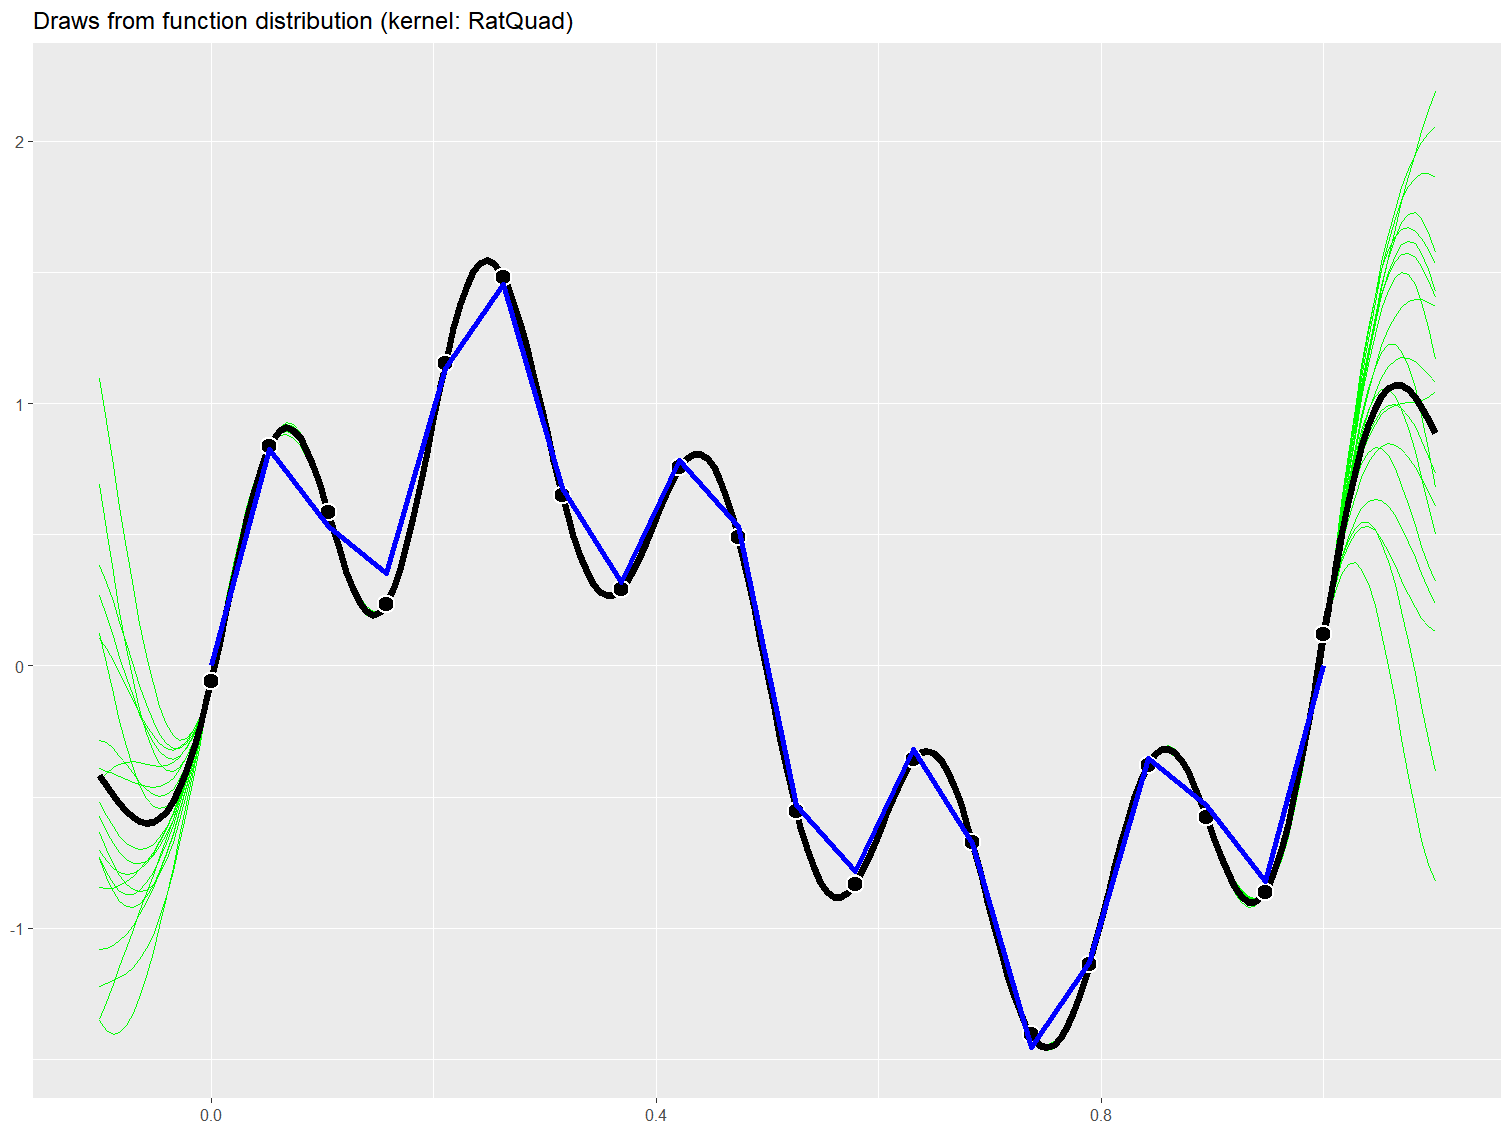
\includegraphics[height=0.5\textwidth]{ratquad_draws.png} \\

% Often causes issues since it assumes infinite differentiability. Experts don’t recommend using it. \cite{gaopro}

\subsubsection{$\gamma$-exponential and exponential}
SE has no parameter that controls or reduce its MS differentiability and its smoothness, rendering it a poor approximation of the less smooth functions we often encounter in the real world. We can introduce a differentiability parameter $\gamma$ to control how differentiable the covariance function is:
\begin{equation*}
    k(X,X') = \exp \left(-\frac{|X - X'|^{\gamma}}{l^{\gamma}} \right)
\end{equation*}
where $0 < \gamma \geq 2$ controls the smoothness of the covariance function. 

\begin{figure}[H]
    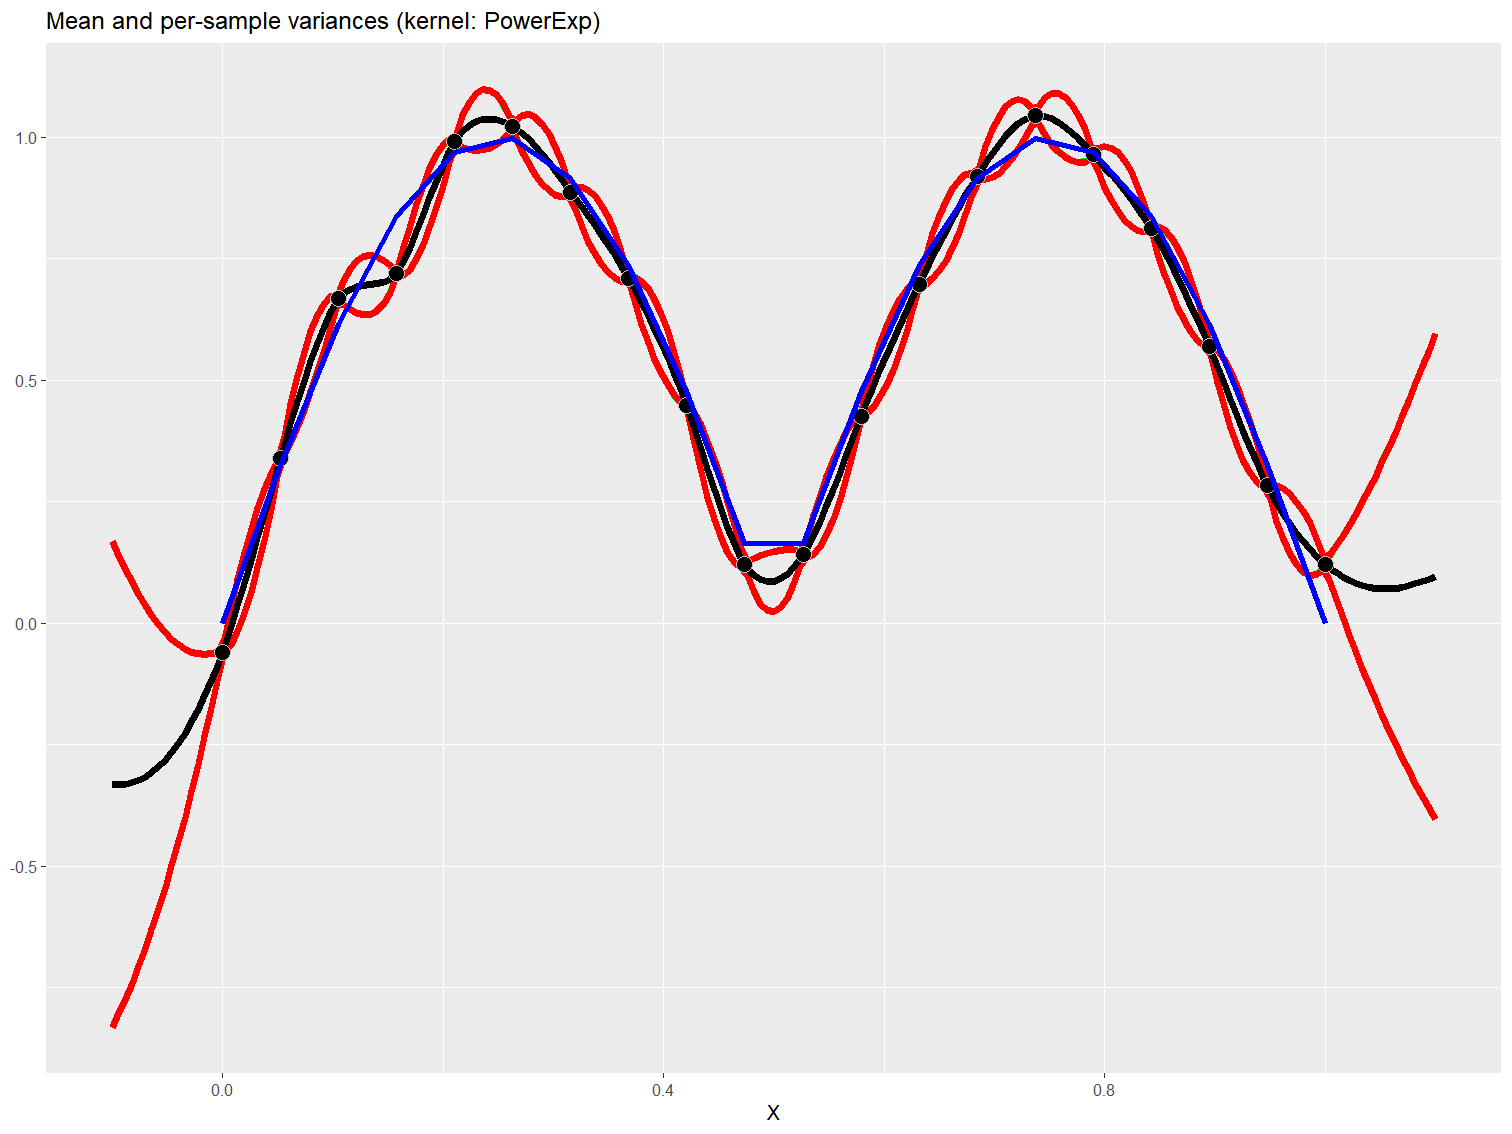
\includegraphics[height=0.5\textwidth]{powerexp_variances.png}
    \caption{
        Plot of a Gaussian process using $\gamma$-exponential applied to the toy dataset. For this dataset, the R package GauPro \cite{gaopro} has used $\gamma = 1.688043$ obtained via MLE. \\
        There are no green lines here because TODO. $\gamma$-exponential produces much rougher functions than SE, so its expected function has a lot more wiggle and conforms to the datapoints much closer than SE. In this case, our data-generating function is smooth so SE is closer to the data-generating function than $\gamma$-exponential, but real world data-generating functions are often much rougher and would benefit from a kernel flexible enough to pass through the datapoints.
    }
\end{figure}

\begin{figure}[H]
    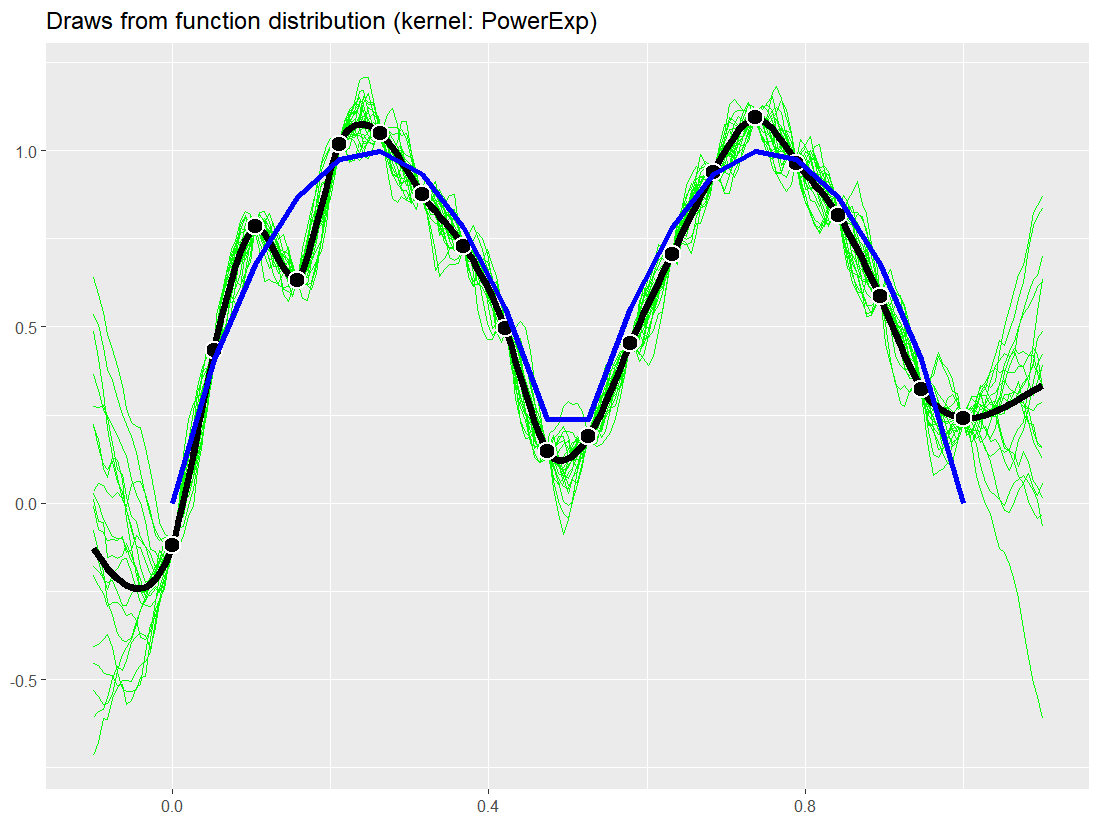
\includegraphics[height=0.5\textwidth]{powerexp_draws.png}
    \caption{
        Plots of functions from a Gaussian process using $\gamma$-exponential applied to the same toy dataset. \\
        These sample function draws are much rougher than SE.
    }
\end{figure}

$\gamma = 2$ produces SE for maximal smoothness, while $\gamma = 1$ produces the exponential covariance function:
\begin{equation*}
    k(X,X') = \exp \left(-\frac{|X - X'|}{l} \right)
\end{equation*}
Here, and for all other values of $\gamma$ other than $2$, the covariance function is continuous but not differentiable at all at $|x - x'| = 0$, which coincides with the undifferentiable turning point of the modulus function at $x - x' = 0$, and produces the roughest functions of all covariance functions we consider.

\begin{figure}[H]
    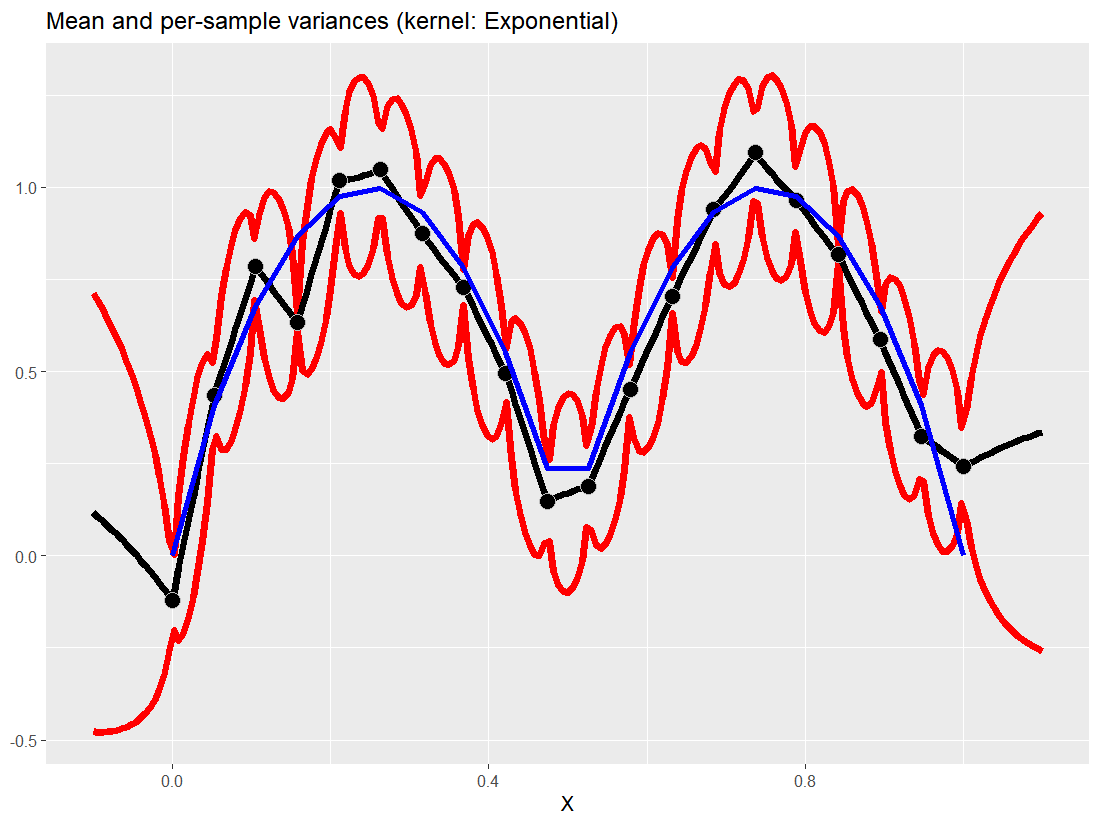
\includegraphics[height=0.5\textwidth]{exp_variances.png}
    \caption{
        Plot of a Gaussian process using exponential applied to the toy dataset. \\
        TODO explain
    }
\end{figure}

\begin{figure}[H]
    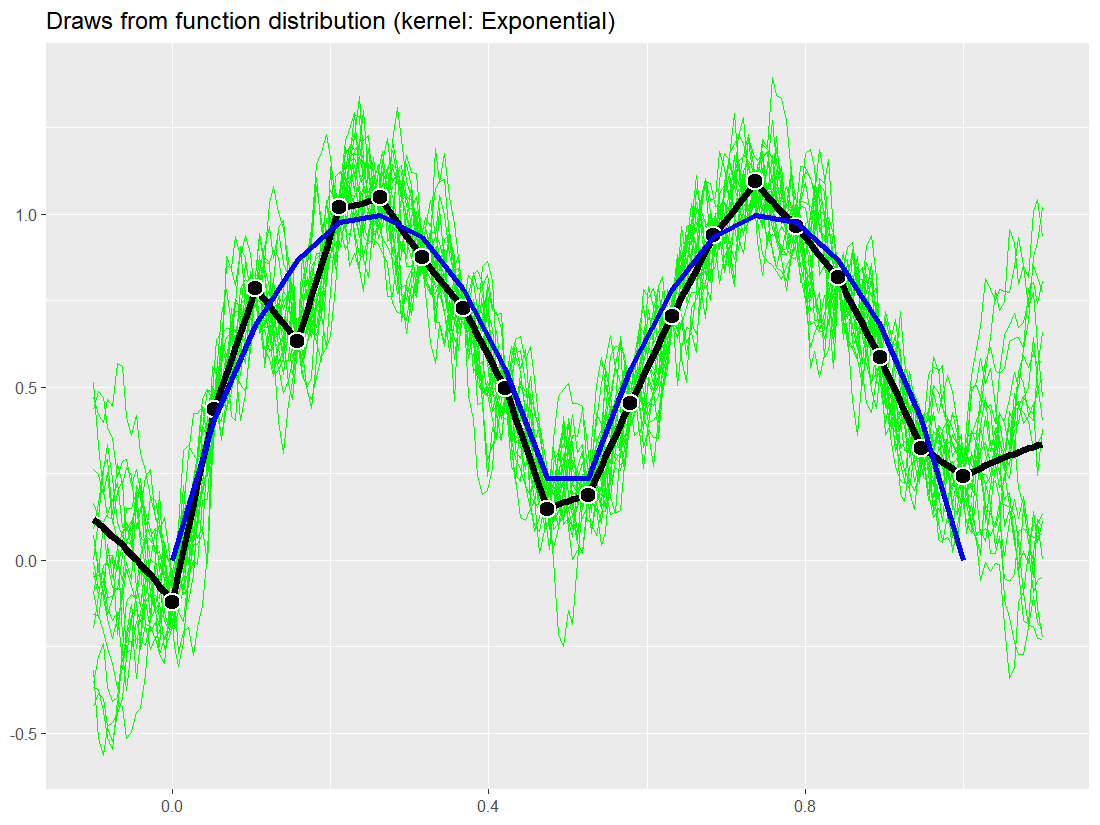
\includegraphics[height=0.5\textwidth]{exp_draws.png}
    \caption{
        Plots of functions from a Gaussian process using exponential applied to the same toy dataset. \\
        These sample function draws are much rougher than SE and $\gamma$-exponential.
    }
\end{figure}


% Exponential: Equivalent to Matern 1/2. Assumes no differentiability. \cite{gaopro}


\subsubsection{Matern-class}
The $\gamma$-exponential generalisation is not useful due to its brittleness - it can only produce two covariance functions representing the extremes of the smoothness-roughness scale. The Matern class of covariance functions addresses this by introducing a parameter $\nu > 0$ that controls the smoothness of the function. The Matern class is defined as:
\begin{equation*}
    k(X,X') = \frac{2^{1 - \nu}}{\Gamma(\nu)}\left(\frac{\sqrt{2\nu}|X - X'|}{l}\right)^{\nu}K_{\nu}\left(\frac{\sqrt{2\nu}|X - X'|}{l}\right)
\end{equation*}

$l$ is our familiar length scale hyperparameter. TODO Bessel function $K_{\nu}$, background needed. Therefore, a Gaussian process using a Matern class kernel is $k$-times MS differentiable if and only if $\nu > k$. 

Using half-integers, i.e. $\nu = p + 1/2$ where $p$ is a non-negative integer, the covariance function becomes a product of a polynomial and an exponential:

\begin{equation*}
    k_{\nu = p + 1/2}(X,X') = \exp \left(- \frac{\sqrt{2\nu}|X - X'|}{l} \right) \frac{\Gamma(p+1)}{\Gamma(2p+1)} \sum_{i=0}^p \frac{(p + i)!}{i!(p-i)!} \left( \frac{\sqrt{8\nu r}}{l} \right)^{p-i}
\end{equation*}

$\nu = 1/2$ is equivelant to the exponential covariance function. As $\nu \to \infty$, the Matern covariance function approaches the SE covariance function. Practically, $\nu \geq 7/2$ produces functions that are as smooth as SE, leaving us with two cases of interest: $\nu = 3/2$ and $\nu = 5/2$.

\paragraph{Matern 3/2}
$\nu = 3/2$ produces the following covariance function:
\begin{equation*}
    k_{3/2}(X,X') = \left(1 + \frac{\sqrt{3}|X - X'|}{l} \right) \exp \left(-\frac{\sqrt{3}|X - X'|}{l} \right)
\end{equation*}
3/2 is one-time MS differentiable, leading to much rougher functions than SE.

\begin{figure}[H]
    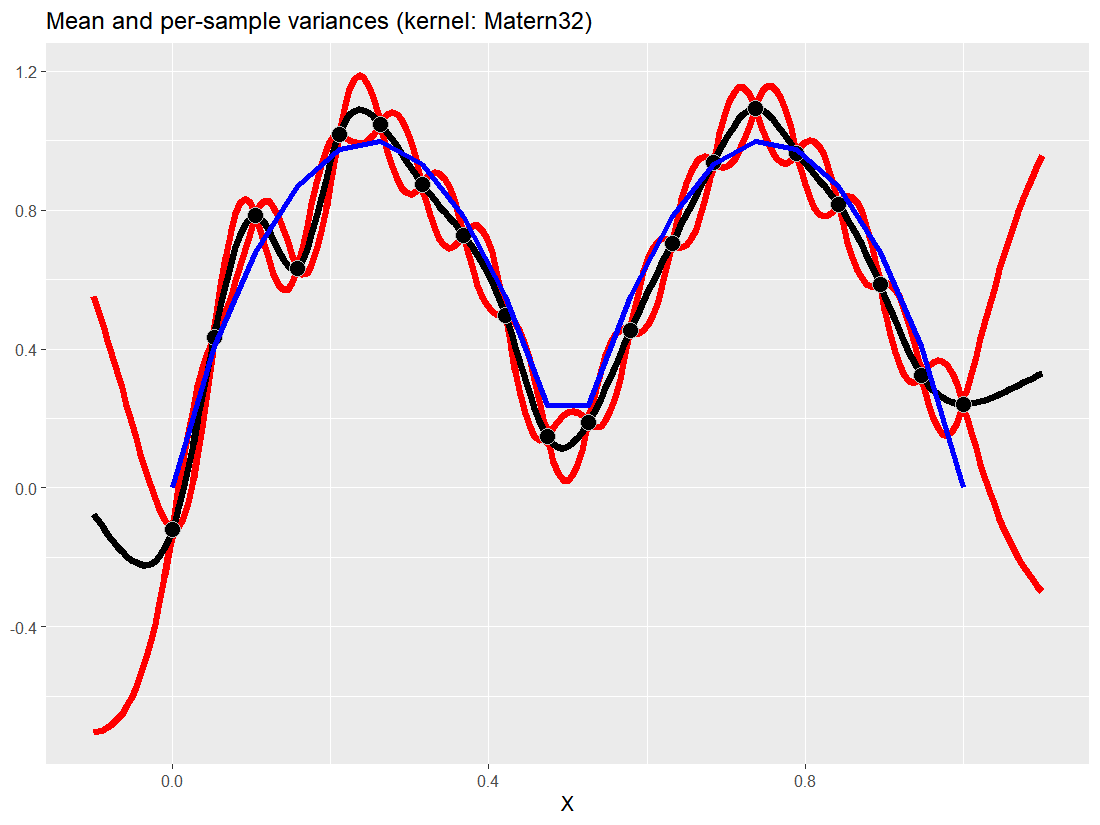
\includegraphics[height=0.5\textwidth]{matern32_variances.png}
    \caption{
        Plot of a Gaussian process using Matern 3/2 applied to the toy dataset. \\
        TODO explain
    }
\end{figure}

\begin{figure}[H]
    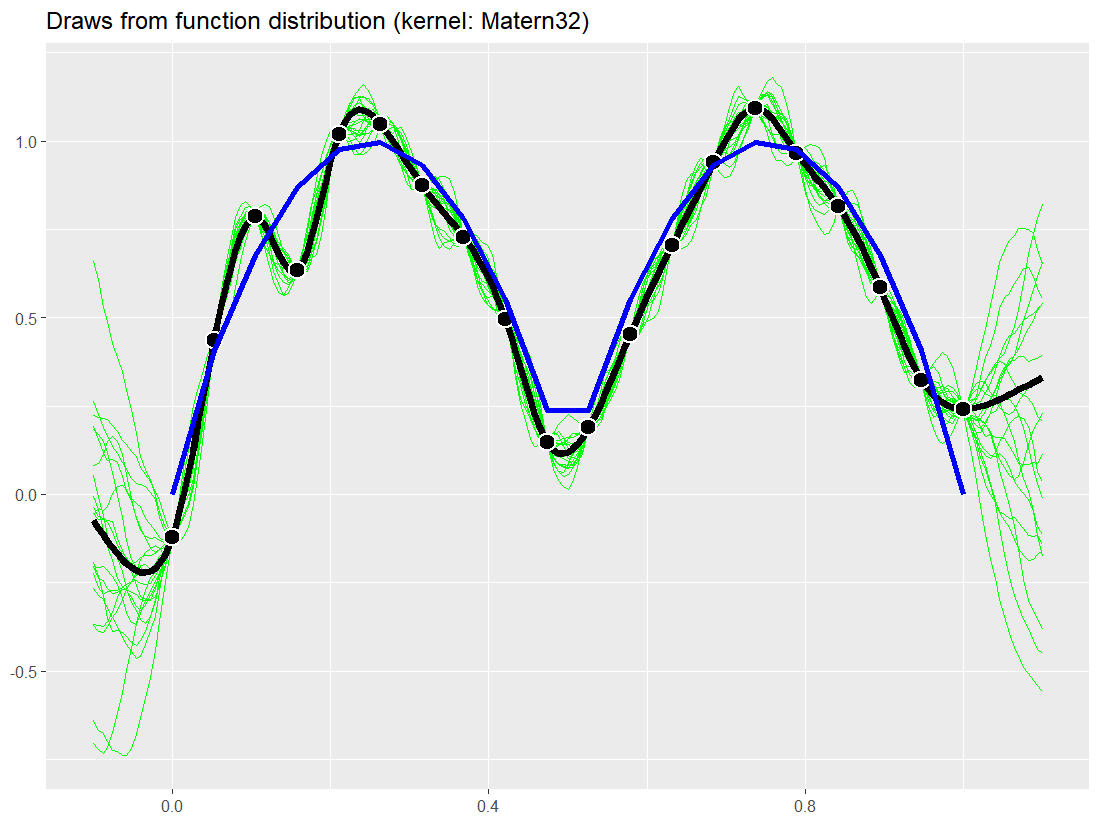
\includegraphics[height=0.5\textwidth]{matern32_draws.png}
    \caption{
        Plots of functions from a Gaussian process using Matern 3/2 applied to the same toy dataset. \\
        TODO explain
    }
\end{figure}

% Matern 3/2: Assumes one time differentiability. This is often too low of an assumption. \cite{gaopro}

\paragraph{Matern 5/2}
$\nu = 5/2$ produces the following covariance function:
\begin{equation*}
    k_{5/2}(X,X') = \left(1 + \frac{\sqrt{5}|X - X'|}{l} + \frac{5|X - X'|^2}{3l^2} \right) \exp \left(-\frac{\sqrt{5}|X - X'|}{l} \right)
\end{equation*}
5/2 is twice MS differentiable, producing functions that are slightly smoother than 3/2.

\begin{figure}[H]
    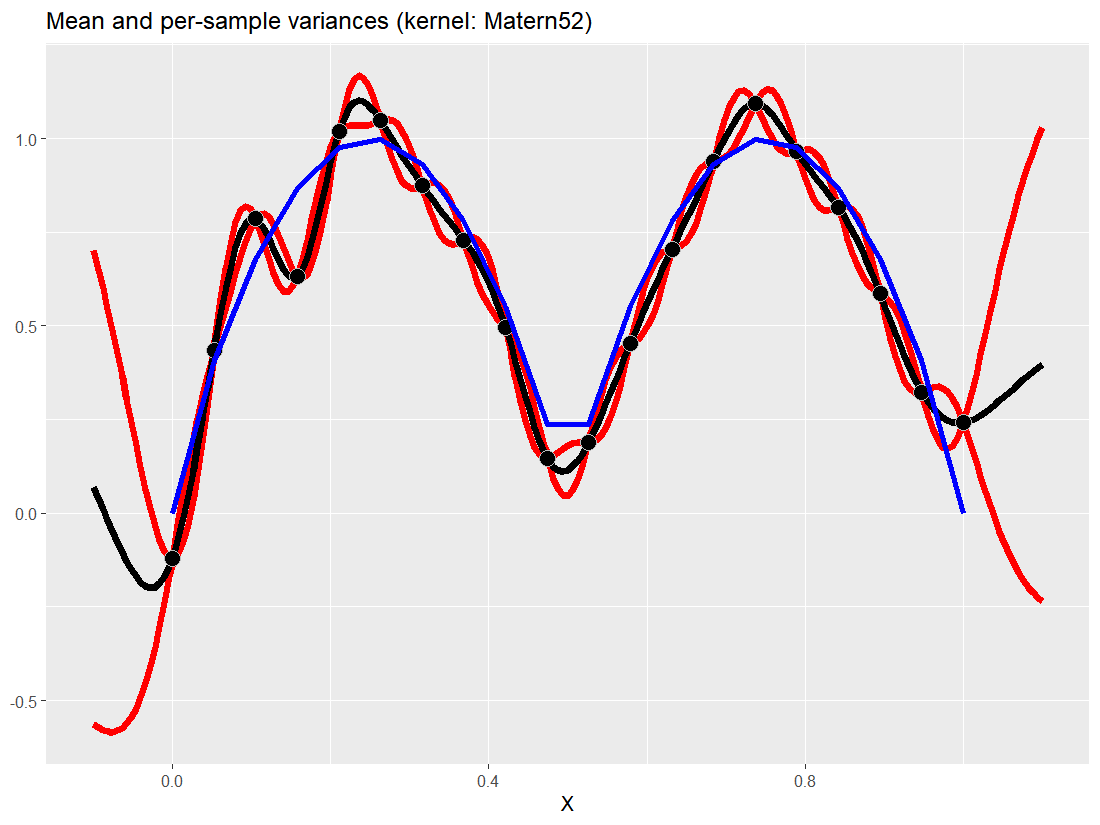
\includegraphics[height=0.5\textwidth]{matern52_variances.png}
    \caption{
        Plot of a Gaussian process using Matern 5/2 applied to the toy dataset. \\
        The expected function deviates very slightly from datapoints compared to 3/2, but the big difference compared to 3/2 is in the variances. 5/2 has narrower variances than 3/2, producing smoother functions and functions that are closer to the expected function. SE is still better in this instance because it is the most smooth and our data-generating function is unusually smooth. However, 5/2 is generally the most popular covariance function because it achieves this parsimonious balance between smoothness, to still reach some reasonable approximation of the data-generating function, and flexibility, to still pass through the datapoints. 
    }
\end{figure}

\begin{figure}[H]
    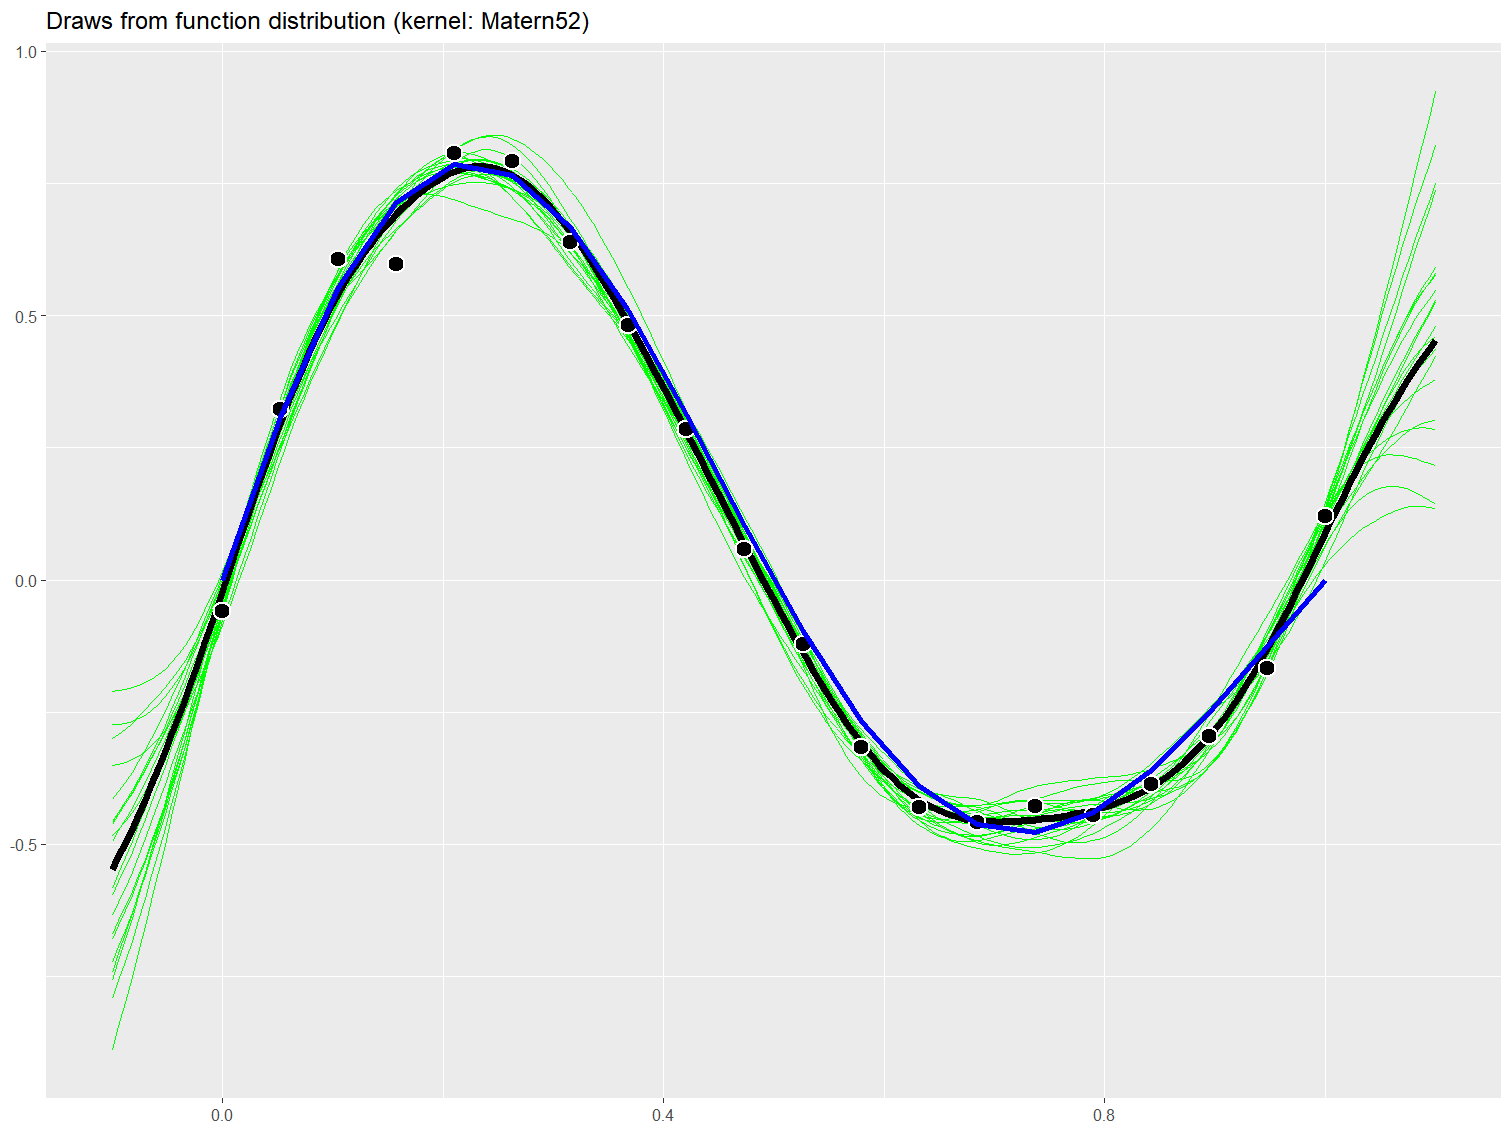
\includegraphics[height=0.5\textwidth]{matern52_draws.png}
    \caption{
        Plots of functions from a Gaussian process using Matern 5/2 applied to the same toy dataset. \\
        These sample function draws conform more to the expected function than 3/2 due to the narrower variances, but are still much rougher than SE and approach the data-points.
    }
\end{figure}

% Matern 5/2: Assumes two time differentiability. Generally the best. \cite{gaopro}




% \subsection{Non-stationary covariance functions \cite{gp-ml}}
% 
% \subsubsection{Sum and product}
% 
% \subsubsection{Neural network}
% 
% \subsubsection{Warping and periodicity}


% \subsection{Language-processing covariance functions \cite{gp-ml}}
% 
% \subsubsection{String}
% 
% \subsubsection{Fisher}
% 
% 
% \subsection{Factor-processing covariance functions \cite{gaopro}}
% 
% \subsubsection{Ordered factor}
% 
% \subsubsection{Factor}
% 
% \subsubsection{Gower factor}
% 
% \subsubsection{Indices-ignoring}


% \subsection{Deriving kernels \cite{deriving-kernels}}
% TODO
% 
% \subsection{Learning best kernel from data \cite{choosing-kernels}}
% TODO

% \subsection{Additive covariance kernels for high-dimensional learning \cite{additive-kernels}}
% 
% 
% \subsection{Hierarchical Bayesian covariance function for hierarchical modelling \cite{hierarchical-kernels}}
% 
% 
% \subsection{Free-form covariance matrix for multi-task learning \cite{freeform-kernels}}
% 
% 
% \subsection{Combining different kernels for multi-task learning \cite{multi-kernels}}



% \section{Extensions of the Gaussian Process}
% 
% 
% \subsection{Gaussian process regression networks \cite{gprn}}
% 
% 
% \subsection{Variational Gaussian process \cite{vgp}}
